\documentclass{extbook}[14pt]
\usepackage{multicol, enumerate, enumitem, hyperref, color, soul, setspace, parskip, fancyhdr, amssymb, amsthm, amsmath, latexsym, units, mathtools}
\everymath{\displaystyle}
\usepackage[headsep=0.5cm,headheight=0cm, left=1 in,right= 1 in,top= 1 in,bottom= 1 in]{geometry}
\usepackage{dashrule}  % Package to use the command below to create lines between items
\newcommand{\litem}[1]{\item #1

\rule{\textwidth}{0.4pt}}
\pagestyle{fancy}
\lhead{}
\chead{Answer Key for Makeup Progress Quiz 2 Version B}
\rhead{}
\lfoot{5763-3522}
\cfoot{}
\rfoot{Spring 2021}
\begin{document}
\textbf{This key should allow you to understand why you choose the option you did (beyond just getting a question right or wrong). \href{https://xronos.clas.ufl.edu/mac1105spring2020/courseDescriptionAndMisc/Exams/LearningFromResults}{More instructions on how to use this key can be found here}.}

\textbf{If you have a suggestion to make the keys better, \href{https://forms.gle/CZkbZmPbC9XALEE88}{please fill out the short survey here}.}

\textit{Note: This key is auto-generated and may contain issues and/or errors. The keys are reviewed after each exam to ensure grading is done accurately. If there are issues (like duplicate options), they are noted in the offline gradebook. The keys are a work-in-progress to give students as many resources to improve as possible.}

\rule{\textwidth}{0.4pt}

\begin{enumerate}\litem{
Construct the lowest-degree polynomial given the zeros below. Then, choose the intervals that contain the coefficients of the polynomial in the form $ax^3+bx^2+cx+d$.
\[ \frac{1}{3}, 7, \text{ and } \frac{5}{3} \]The solution is \( 9x^{3} -81 x^{2} +131 x -35 \), which is option A.\begin{enumerate}[label=\Alph*.]
\item \( a \in [2, 13], b \in [-83, -77], c \in [129, 133], \text{ and } d \in [-38, -33] \)

* $9x^{3} -81 x^{2} +131 x -35$, which is the correct option.
\item \( a \in [2, 13], b \in [-83, -77], c \in [129, 133], \text{ and } d \in [35, 38] \)

$9x^{3} -81 x^{2} +131 x + 35$, which corresponds to multiplying everything correctly except the constant term.
\item \( a \in [2, 13], b \in [79, 93], c \in [129, 133], \text{ and } d \in [35, 38] \)

$9x^{3} +81 x^{2} +131 x + 35$, which corresponds to multiplying out $(3x + 1)(x + 7)(3x + 5)$.
\item \( a \in [2, 13], b \in [-77, -74], c \in [79, 80], \text{ and } d \in [35, 38] \)

$9x^{3} -75 x^{2} +79 x + 35$, which corresponds to multiplying out $(3x + 1)(x -7)(3x -5)$.
\item \( a \in [2, 13], b \in [51, 52], c \in [-90, -84], \text{ and } d \in [-38, -33] \)

$9x^{3} +51 x^{2} -89 x -35$, which corresponds to multiplying out $(3x + 1)(x + 7)(3x -5)$.
\end{enumerate}

\textbf{General Comment:} To construct the lowest-degree polynomial, you want to multiply out $(3x -1)(x -7)(3x -5)$
}
\litem{
Construct the lowest-degree polynomial given the zeros below. Then, choose the intervals that contain the coefficients of the polynomial in the form $x^3+bx^2+cx+d$.
\[ 4 - 5 i \text{ and } 1 \]The solution is \( x^{3} -9 x^{2} +49 x -41 \), which is option D.\begin{enumerate}[label=\Alph*.]
\item \( b \in [1, 3], c \in [-11, -4], \text{ and } d \in [2, 9] \)

$x^{3} + x^{2} -5 x + 4$, which corresponds to multiplying out $(x -4)(x -1)$.
\item \( b \in [5, 20], c \in [49, 51], \text{ and } d \in [38, 46] \)

$x^{3} +9 x^{2} +49 x + 41$, which corresponds to multiplying out $(x-(4 - 5 i))(x-(4 + 5 i))(x + 1)$.
\item \( b \in [1, 3], c \in [0, 9], \text{ and } d \in [-11, 2] \)

$x^{3} + x^{2} +4 x -5$, which corresponds to multiplying out $(x + 5)(x -1)$.
\item \( b \in [-17, -5], c \in [49, 51], \text{ and } d \in [-44, -38] \)

* $x^{3} -9 x^{2} +49 x -41$, which is the correct option.
\item \( \text{None of the above.} \)

This corresponds to making an unanticipated error or not understanding how to use nonreal complex numbers to create the lowest-degree polynomial. If you chose this and are not sure what you did wrong, please contact the coordinator for help.
\end{enumerate}

\textbf{General Comment:} Remember that the conjugate of $a+bi$ is $a-bi$. Since these zeros always come in pairs, we need to multiply out $(x-(4 - 5 i))(x-(4 + 5 i))(x-(1))$.
}
\litem{
Which of the following equations \textit{could} be of the graph presented below?

\begin{center}
    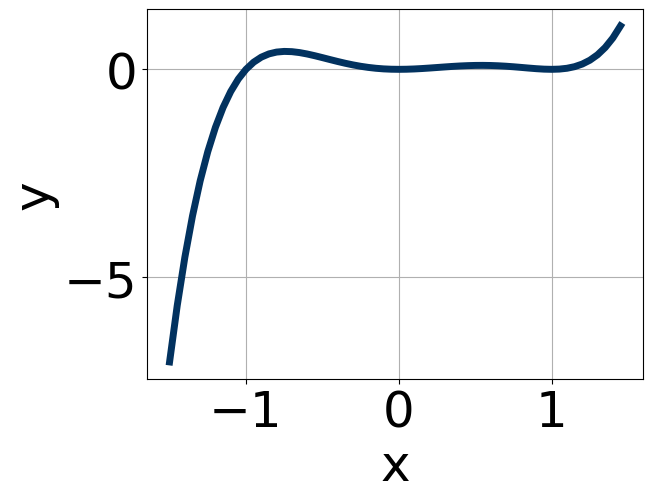
\includegraphics[width=0.5\textwidth]{../Figures/polyGraphToFunctionB.png}
\end{center}


The solution is \( 8x^{4} (x - 1)^{4} (x + 1)^{5} \), which is option E.\begin{enumerate}[label=\Alph*.]
\item \( 9x^{9} (x - 1)^{8} (x + 1)^{11} \)

The factor $x$ should have an even power.
\item \( -9x^{8} (x - 1)^{8} (x + 1)^{7} \)

This corresponds to the leading coefficient being the opposite value than it should be.
\item \( -20x^{8} (x - 1)^{4} (x + 1)^{4} \)

The factor $(x + 1)$ should have an odd power and the leading coefficient should be the opposite sign.
\item \( 8x^{9} (x - 1)^{8} (x + 1)^{6} \)

The factor $x$ should have an even power and the factor $(x + 1)$ should have an odd power.
\item \( 8x^{4} (x - 1)^{4} (x + 1)^{5} \)

* This is the correct option.
\end{enumerate}

\textbf{General Comment:} General Comments: Draw the x-axis to determine which zeros are touching (and so have even multiplicity) or cross (and have odd multiplicity).
}
\litem{
Describe the zero behavior of the zero $x = -4$ of the polynomial below.
\[ f(x) = 8(x + 4)^{9}(x - 4)^{12}(x - 7)^{5}(x + 7)^{9} \]The solution is the graph below, which is option A.
\begin{center}
    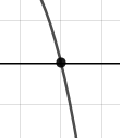
\includegraphics[width=0.3\textwidth]{../Figures/polyZeroBehaviorCopyAB.png}
\end{center}\begin{enumerate}[label=\Alph*.]
\begin{multicols}{2}
\item 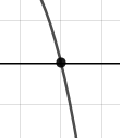
\includegraphics[width = 0.3\textwidth]{../Figures/polyZeroBehaviorCopyAB.png}
\item 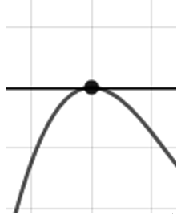
\includegraphics[width = 0.3\textwidth]{../Figures/polyZeroBehaviorCopyBB.png}
\item 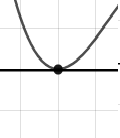
\includegraphics[width = 0.3\textwidth]{../Figures/polyZeroBehaviorCopyCB.png}
\item 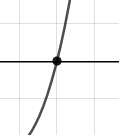
\includegraphics[width = 0.3\textwidth]{../Figures/polyZeroBehaviorCopyDB.png}
\end{multicols}\item None of the above.\end{enumerate}
\textbf{General Comment:} You will need to sketch the entire graph, then zoom in on the zero the question asks about.
}
\litem{
Describe the zero behavior of the zero $x = -8$ of the polynomial below.
\[ f(x) = 3(x + 6)^{6}(x - 6)^{2}(x - 8)^{9}(x + 8)^{6} \]The solution is the graph below, which is option B.
\begin{center}
    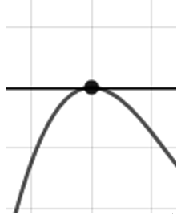
\includegraphics[width=0.3\textwidth]{../Figures/polyZeroBehaviorBB.png}
\end{center}\begin{enumerate}[label=\Alph*.]
\begin{multicols}{2}
\item 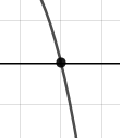
\includegraphics[width = 0.3\textwidth]{../Figures/polyZeroBehaviorAB.png}
\item 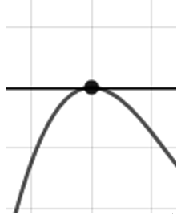
\includegraphics[width = 0.3\textwidth]{../Figures/polyZeroBehaviorBB.png}
\item 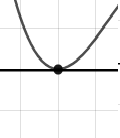
\includegraphics[width = 0.3\textwidth]{../Figures/polyZeroBehaviorCB.png}
\item 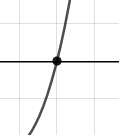
\includegraphics[width = 0.3\textwidth]{../Figures/polyZeroBehaviorDB.png}
\end{multicols}\item None of the above.\end{enumerate}
\textbf{General Comment:} You will need to sketch the entire graph, then zoom in on the zero the question asks about.
}
\litem{
Construct the lowest-degree polynomial given the zeros below. Then, choose the intervals that contain the coefficients of the polynomial in the form $x^3+bx^2+cx+d$.
\[ -5 + 5 i \text{ and } 2 \]The solution is \( x^{3} +8 x^{2} +30 x -100 \), which is option C.\begin{enumerate}[label=\Alph*.]
\item \( b \in [-5, 6], c \in [-9, 1], \text{ and } d \in [7, 22] \)

$x^{3} + x^{2} -7 x + 10$, which corresponds to multiplying out $(x -5)(x -2)$.
\item \( b \in [-12, -2], c \in [29, 38], \text{ and } d \in [92, 102] \)

$x^{3} -8 x^{2} +30 x + 100$, which corresponds to multiplying out $(x-(-5 + 5 i))(x-(-5 - 5 i))(x + 2)$.
\item \( b \in [6, 14], c \in [29, 38], \text{ and } d \in [-106, -99] \)

* $x^{3} +8 x^{2} +30 x -100$, which is the correct option.
\item \( b \in [-5, 6], c \in [-1, 4], \text{ and } d \in [-21, -9] \)

$x^{3} + x^{2} +3 x -10$, which corresponds to multiplying out $(x + 5)(x -2)$.
\item \( \text{None of the above.} \)

This corresponds to making an unanticipated error or not understanding how to use nonreal complex numbers to create the lowest-degree polynomial. If you chose this and are not sure what you did wrong, please contact the coordinator for help.
\end{enumerate}

\textbf{General Comment:} Remember that the conjugate of $a+bi$ is $a-bi$. Since these zeros always come in pairs, we need to multiply out $(x-(-5 + 5 i))(x-(-5 - 5 i))(x-(2))$.
}
\litem{
Construct the lowest-degree polynomial given the zeros below. Then, choose the intervals that contain the coefficients of the polynomial in the form $ax^3+bx^2+cx+d$.
\[ \frac{1}{4}, 7, \text{ and } \frac{-7}{5} \]The solution is \( 20x^{3} -117 x^{2} -168 x + 49 \), which is option A.\begin{enumerate}[label=\Alph*.]
\item \( a \in [20, 22], b \in [-122, -116], c \in [-170, -163], \text{ and } d \in [46, 52] \)

* $20x^{3} -117 x^{2} -168 x + 49$, which is the correct option.
\item \( a \in [20, 22], b \in [165, 181], c \in [238, 243], \text{ and } d \in [46, 52] \)

$20x^{3} +173 x^{2} +238 x + 49$, which corresponds to multiplying out $(4x + 1)(x + 7)(5x + 7)$.
\item \( a \in [20, 22], b \in [-109, -104], c \in [-227, -217], \text{ and } d \in [-53, -44] \)

$20x^{3} -107 x^{2} -224 x -49$, which corresponds to multiplying out $(4x + 1)(x -7)(5x + 7)$.
\item \( a \in [20, 22], b \in [114, 125], c \in [-170, -163], \text{ and } d \in [-53, -44] \)

$20x^{3} +117 x^{2} -168 x -49$, which corresponds to multiplying out $(4x + 1)(x + 7)(5x -7)$.
\item \( a \in [20, 22], b \in [-122, -116], c \in [-170, -163], \text{ and } d \in [-53, -44] \)

$20x^{3} -117 x^{2} -168 x -49$, which corresponds to multiplying everything correctly except the constant term.
\end{enumerate}

\textbf{General Comment:} To construct the lowest-degree polynomial, you want to multiply out $(4x -1)(x -7)(5x + 7)$
}
\litem{
Describe the end behavior of the polynomial below.
\[ f(x) = 7(x + 4)^{3}(x - 4)^{8}(x - 5)^{4}(x + 5)^{4} \]The solution is the graph below, which is option D.
\begin{center}
    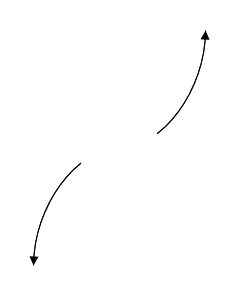
\includegraphics[width=0.3\textwidth]{../Figures/polyEndBehaviorCopyDB.png}
\end{center}\begin{enumerate}[label=\Alph*.]
\begin{multicols}{2}
\item 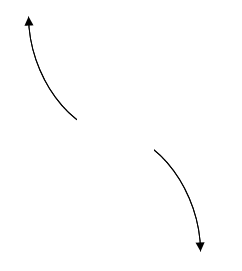
\includegraphics[width = 0.3\textwidth]{../Figures/polyEndBehaviorCopyAB.png}
\item 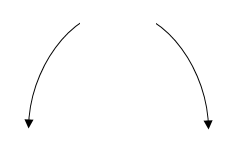
\includegraphics[width = 0.3\textwidth]{../Figures/polyEndBehaviorCopyBB.png}
\item 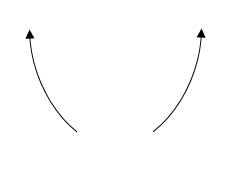
\includegraphics[width = 0.3\textwidth]{../Figures/polyEndBehaviorCopyCB.png}
\item 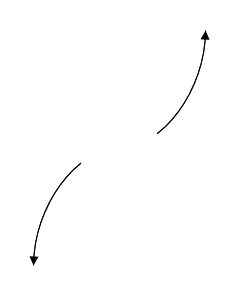
\includegraphics[width = 0.3\textwidth]{../Figures/polyEndBehaviorCopyDB.png}
\end{multicols}\item None of the above.\end{enumerate}
\textbf{General Comment:} Remember that end behavior is determined by the leading coefficient AND whether the \textbf{sum} of the multiplicities is positive or negative.
}
\litem{
Which of the following equations \textit{could} be of the graph presented below?

\begin{center}
    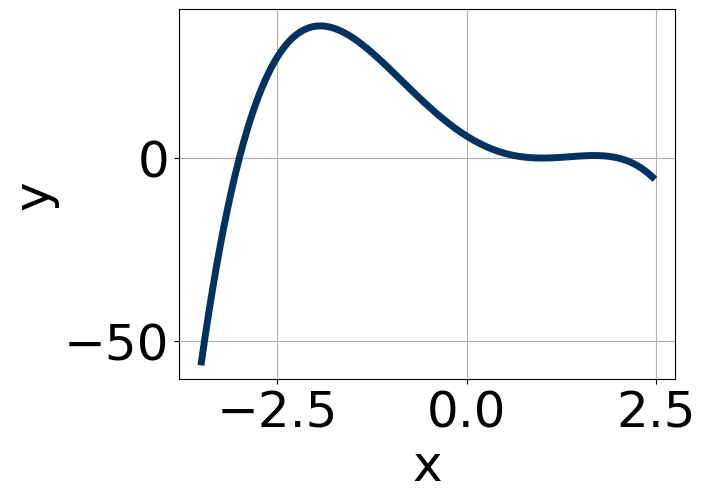
\includegraphics[width=0.5\textwidth]{../Figures/polyGraphToFunctionCopyB.png}
\end{center}


The solution is \( -4(x - 1)^{4} (x + 3)^{5} (x - 2)^{9} \), which is option E.\begin{enumerate}[label=\Alph*.]
\item \( -5(x - 1)^{10} (x + 3)^{6} (x - 2)^{9} \)

The factor $(x + 3)$ should have an odd power.
\item \( 3(x - 1)^{10} (x + 3)^{9} (x - 2)^{6} \)

The factor $(x - 2)$ should have an odd power and the leading coefficient should be the opposite sign.
\item \( -3(x - 1)^{11} (x + 3)^{6} (x - 2)^{9} \)

The factor $1$ should have an even power and the factor $-3$ should have an odd power.
\item \( 18(x - 1)^{6} (x + 3)^{9} (x - 2)^{5} \)

This corresponds to the leading coefficient being the opposite value than it should be.
\item \( -4(x - 1)^{4} (x + 3)^{5} (x - 2)^{9} \)

* This is the correct option.
\end{enumerate}

\textbf{General Comment:} General Comments: Draw the x-axis to determine which zeros are touching (and so have even multiplicity) or cross (and have odd multiplicity).
}
\litem{
Describe the end behavior of the polynomial below.
\[ f(x) = 9(x - 6)^{2}(x + 6)^{3}(x + 8)^{5}(x - 8)^{7} \]The solution is the graph below, which is option D.
\begin{center}
    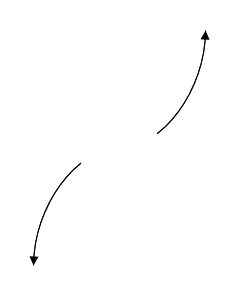
\includegraphics[width=0.3\textwidth]{../Figures/polyEndBehaviorDB.png}
\end{center}\begin{enumerate}[label=\Alph*.]
\begin{multicols}{2}
\item 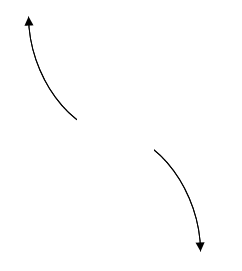
\includegraphics[width = 0.3\textwidth]{../Figures/polyEndBehaviorAB.png}
\item 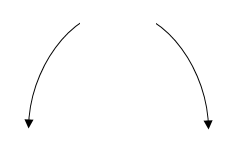
\includegraphics[width = 0.3\textwidth]{../Figures/polyEndBehaviorBB.png}
\item 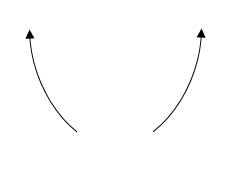
\includegraphics[width = 0.3\textwidth]{../Figures/polyEndBehaviorCB.png}
\item 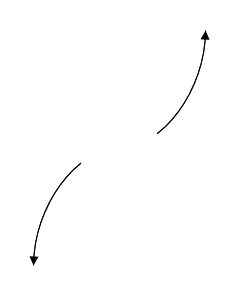
\includegraphics[width = 0.3\textwidth]{../Figures/polyEndBehaviorDB.png}
\end{multicols}\item None of the above.\end{enumerate}
\textbf{General Comment:} Remember that end behavior is determined by the leading coefficient AND whether the \textbf{sum} of the multiplicities is positive or negative.
}
\end{enumerate}

\end{document}